Удобным для интерпретации является построение трехкристальных карт в обратном пространстве.  Таким
образом мы становимся не зависимыми от наличия разных типов дифрактометров, в одних из которых
формирование главного пика осуществляется поворотом образца и поворотом на двойной угол анализатора (ТРС),
в других же дифрактометрах (Rigaku) образец в процессе такого сканирования остается в статичном положении,
а поворачивается источник и детектор на одинаковые углы. Угловые положения падающего пучка и анализатора
определяет вектор рассеяния $\vec{q}$, такой вектор можно разложить на составляющие: $q_z$ - вертикальную составляющую,
направленную перпендикулярно от поверхности отражающей плоскости и $q_x$ - горизонтальную составляющую,
лежащую в отражающей плоскости (рисунок \ref{ris:q_vector_reciprocal_space}).

\begin{figure}[H]
  \centering
  \subfloat[Точное бреговское положение]{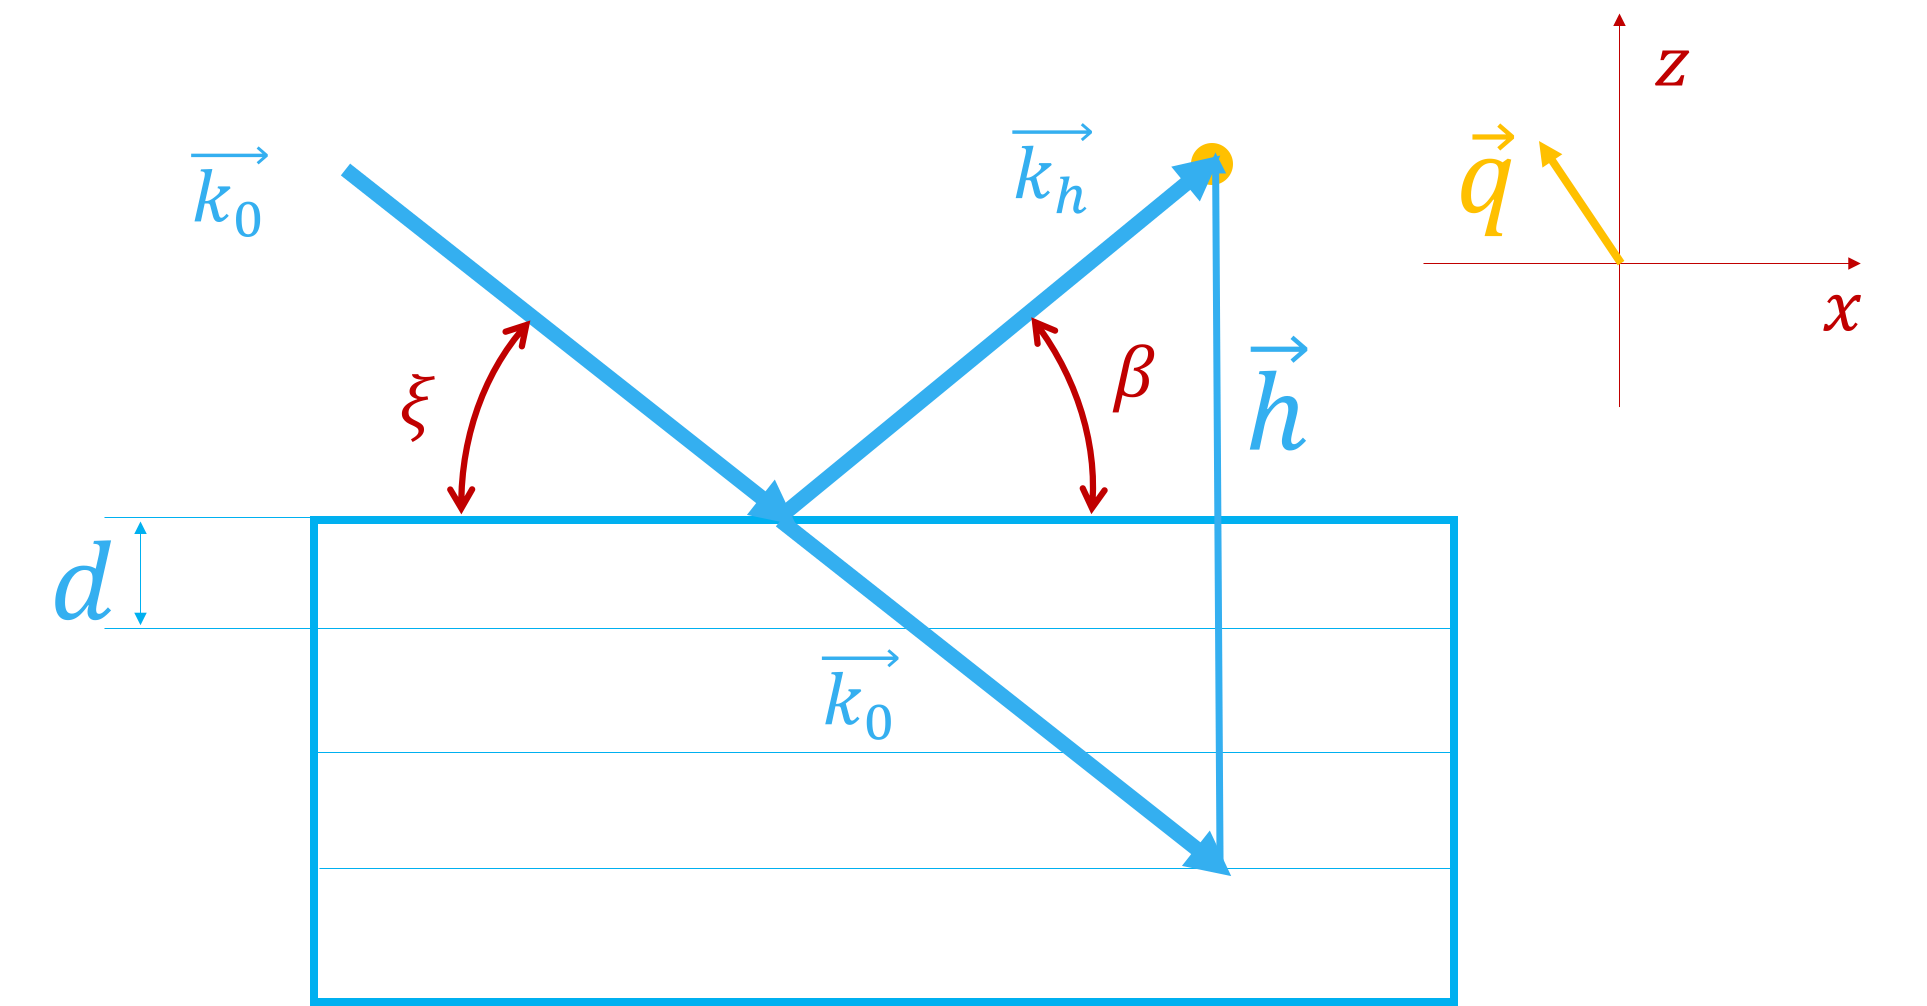
\includegraphics[width=0.3\textwidth]{images/q_vector/0.png}}
  \hfill
  \subfloat[Около брегговское положение - деформация]{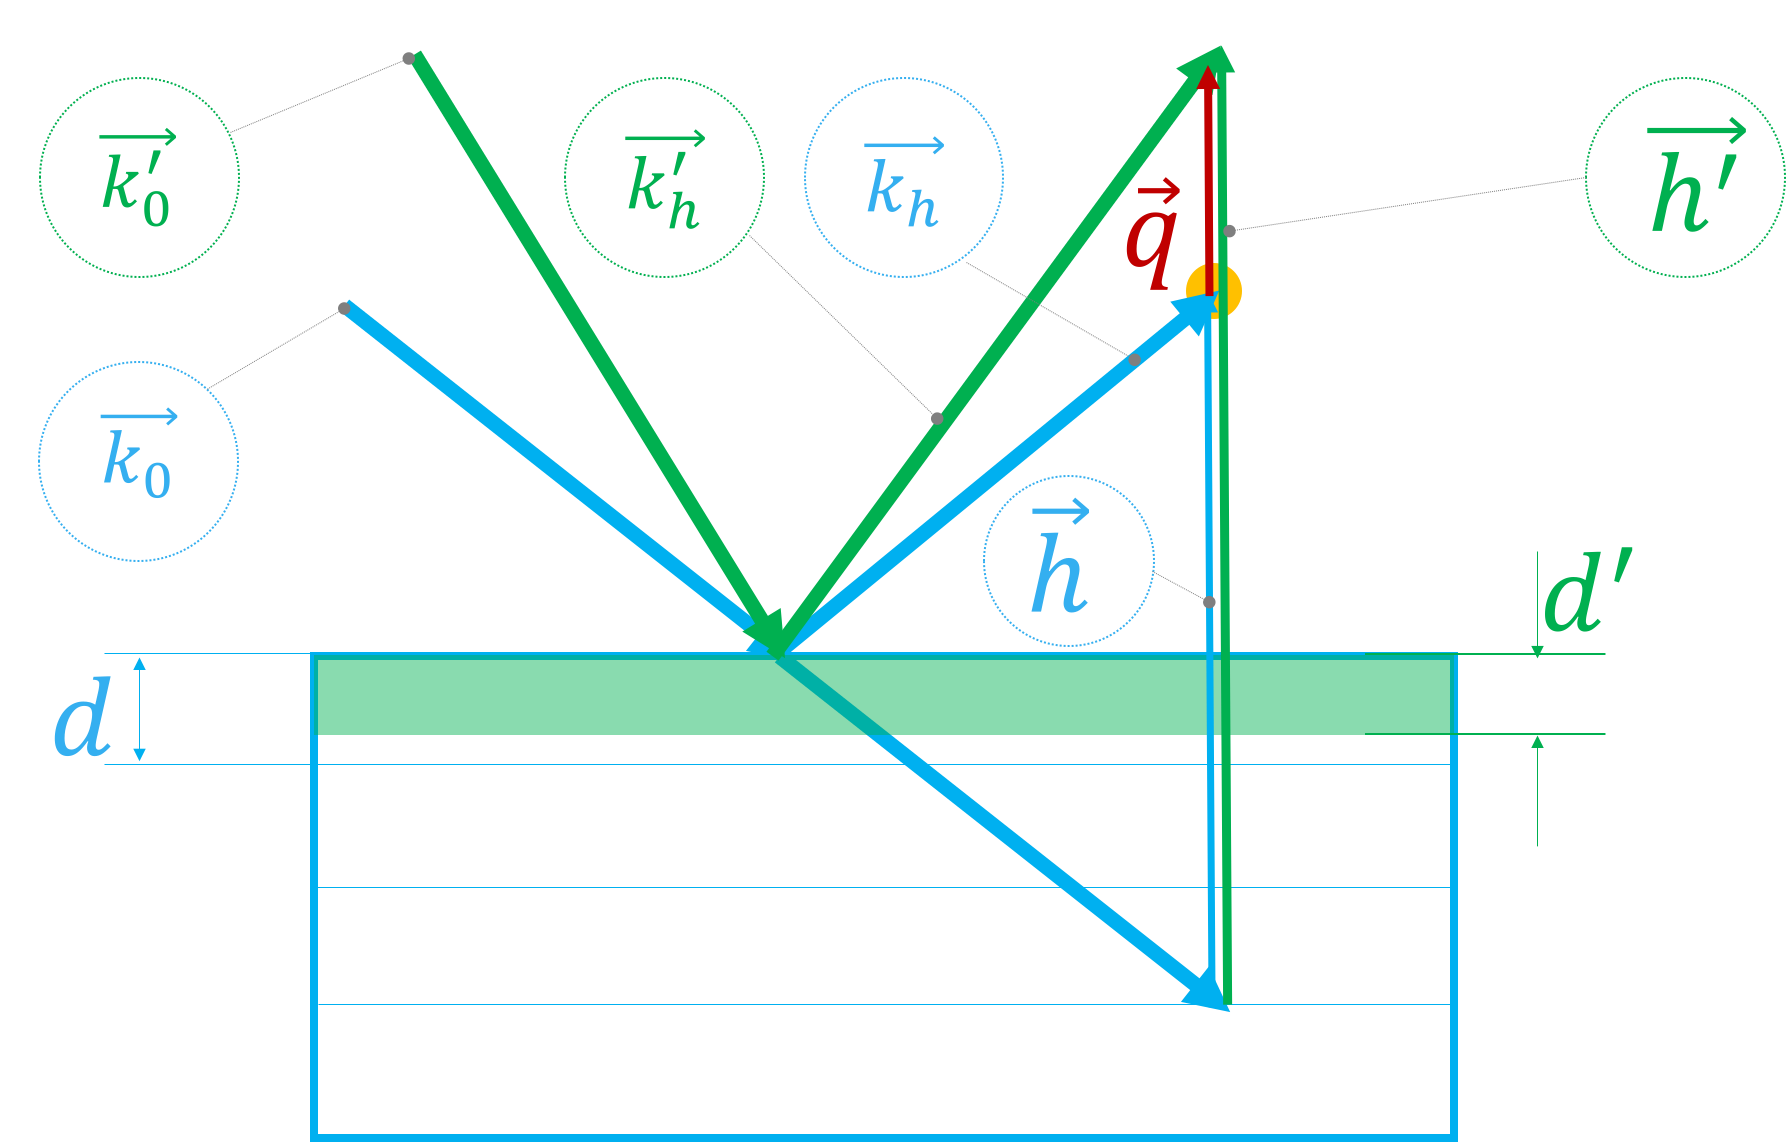
\includegraphics[width=0.3\textwidth]{images/q_vector/_1.png}}
  \hfill
  \subfloat[Около брегговское положение - разориентация]{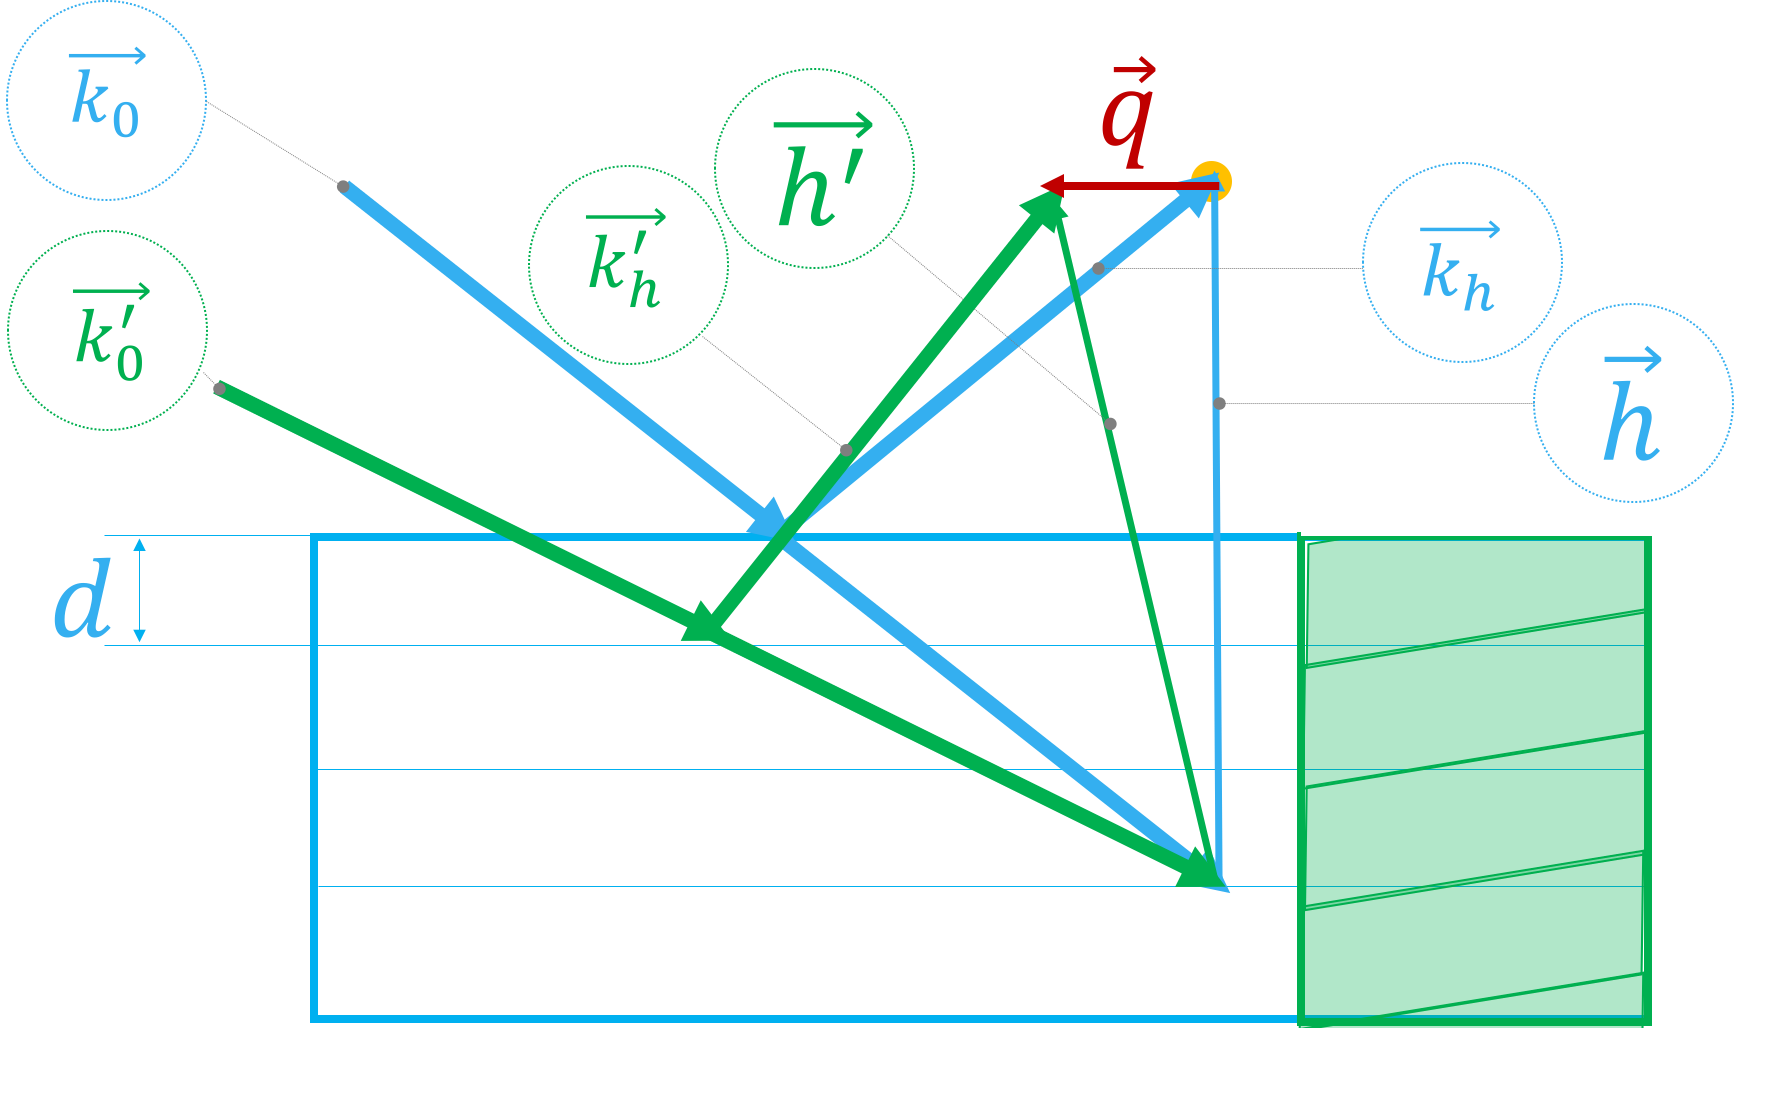
\includegraphics[width=0.3\textwidth]{images/q_vector/1.png}}
  \caption{Отклонение вектора обратной решетки от точного положения}
  \label{ris:q_vector_reciprocal_space}
\end{figure}

Для симметричного отражения эти составляющие связаны с отклонением образца $\theta$ и
анализатора $\varepsilon$ от нулевых положений в номинальном угле Брегга следующими
уравнениями \cite{Tanner_1998}:

\begin{equation}
  q_x = \frac{\varepsilon}{|\vec{k}_0|} \cos \theta_B
  \label{eq:qx_eqn}
\end{equation}

\begin{equation}
  q_z = \frac{2\theta - \varepsilon}{|\vec{k}_0|} \sin \theta_B
  \label{eq:qz_eqn}
\end{equation}

Таким образом, сканирование образцом влияет только на $q_y$ - слева направо в обратном пространстве.
Сканирование анализатора влияет на оба вектора, изменение только одного $q_z$ достигается за
счет $\theta-2\theta$ сканирования.

\begin{figure}[H]
  \centering
  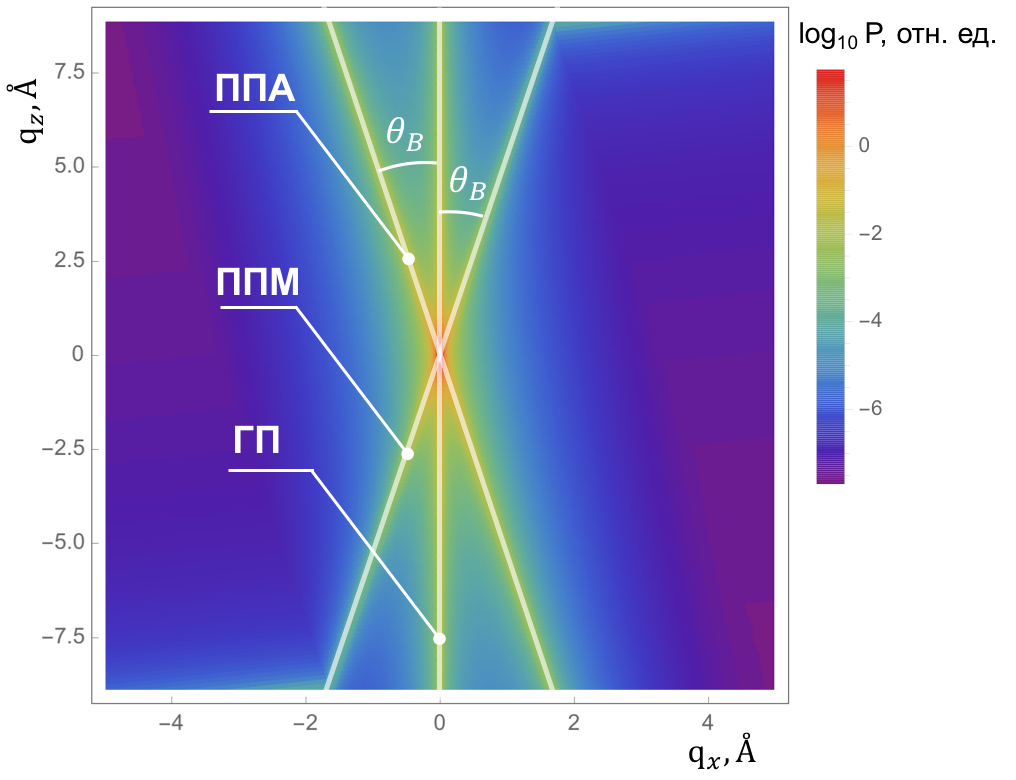
\includegraphics[width=0.6\textwidth]{images/triple_map_reciprocal_space.png}
  \caption{Карта рассеяния в обратном пространстве}
  \label{ris:triple_map_reciprocal_space}
\end{figure}

Угол между ГП и ПП определяется исходя из соотношений (\ref{eq:qx_eqn}, \ref{eq:qz_eqn}) и равен углу Брегга образца:

\begin{equation}
  \frac{q_y}{q_z} = \frac{2\theta - \varepsilon}{\varepsilon} \cdot \tan (\theta_B) = \pm \tan (\theta_B)
  \label{eq:qz_eqn}
\end{equation}
